%%%%%%%%%%%%%%%%%%%%%%%%
% Sample use of the infthesis class to prepare an MSc thesis.
% This can be used as a template to produce your own thesis.
% Date: June 2019
%
%
% The first line specifies style options for taught MSc.
% You should add a final option specifying your degree.
% *Do not* change or add any other options.
%
% So, pick one of the following:
% \documentclass[msc,deptreport,adi]{infthesis}     % Adv Design Inf
 \documentclass[msc,deptreport,ai]{infthesis}      % AI
% \documentclass[msc,deptreport,cogsci]{infthesis}  % Cognitive Sci
% \documentclass[msc,deptreport,cs]{infthesis}      % Computer Sci
% \documentclass[msc,deptreport,cyber]{infthesis}   % Cyber Sec
% \documentclass[msc,deptreport,datasci]{infthesis} % Data Sci
% \documentclass[msc,deptreport,di]{infthesis}      % Design Inf
% \documentclass[msc,deptreport,inf]{infthesis}     % Informatics
%%%%%%%%%%%%%%%%%%%%%%%%

%\documentclass[msc,deptreport]{infthesis} % Do not change except to add your degree (see above).
\usepackage{yfonts}
\usepackage[pdftex]{graphicx}  
\usepackage{float}
\usepackage{url}
\usepackage{fancyvrb}

\begin{document}
\begin{preliminary}

\title{Building a database to store Protein-Protein Interactions (PPI) in a rule based format}

\author{Ayush Das}

\abstract{
The study of Protein-Protein interactions (PPI) involves the analysis and identification of complexes that may form under a variety of reaction conditions. These reactions were initially modeled as Ordinary Differential Equations (ODEs) \cite{ode}, which is now progressing to a rule-based modeling approach. This is because the interacting biomolecules have the potential to interact in a myriad different ways. The number of possible post-translational modifications and complexes grow exponentially when considering the binary interactions within the reaction network. Using traditional methods like ODEs to model PPI requires large amounts of reaction specific details, and the chemical kinetics of the interactions within network requires explicit mention of the network conditions \cite{rule-based-general}. A rule-based model on the other hand comprises of, a set of rules where the network specification is implicit. These rules can specified using model specification languages like Kappa \cite{kappa} or BioNetGen \cite{bioNetGen}. Software tools enable researchers to model these interactions using different objectives like deterministic or stochastic modeling. Hence, researchers in bioinformatics have spent tremendous efforts in collecting the Protein-Protein interaction rules and the purpose of this project is to create and load a database with the PPI rules stored in a rule-based format. This will enable researchers to readily access PPI rules which when fed to a  simulator will enable study of the protein interactions and draw conclusions based on their observations.

% Cite BioNetGen
% Cite Kappa
% Cite  ODE
% Cite the first paper
}

\maketitle

\section*{Acknowledgements}
I would like to thank my supervisor Oksana Sorokina for her continued guidance and support during all stages of this project. The insightful feedback and guidance helped in improving the project to a large extent. I would also like to thank, Anatoly Sorokin and Douglas Armstrong for their insightful feedback and support during the course of this project.

Finally, I would like to thank my family for their support and guidance.

\tableofcontents
\end{preliminary}


\chapter{Introduction}
Protein is an important component of the cells in the human body. It is an important component of bones, muscles, cartilage and so on. Decades of research in the field of biology have produced a vast repository of knowledge on individual protein molecules. Examples of such knowledge base include UniProt \cite{uniprot}. However, in order to further explore the relationships of complex molecular species it is imperative to understand the interactions that take place between them and their governing rules.

As per \cite{ppiDef} Protein-Protein Interactions (PPI) are defined as the physical contacts with molecular docking between the protein molecules that occur in a living organism or cell. PPI interactions play a vital role as they dictate cellular activities which are responsible for good health or diseases. Achieving an in-depth understanding of protein interactions will help researchers improve the existing quality of medicine and health care in general. According to \cite{ppimp} an important source for drug discovery is the study of PPI. This is also evident from the fact that, as per \cite{cancer} in recent times the study of PPI has gained momentum for research in the field of anti-cancer therapy. All these facts suggest the importance of PPI and it's applications. 

Known PPIs are stored in PPI repositories designed to be easily retrievable by the researchers based on the relevant search term. There have been several databases in the past that have tackled the problem of collecting the PPIs. Such databases are of different varieties, based on their method of organizing and structuring the data. These kinds of databases are covered in greater detail, in Chapter 2. 

PPI interactions are used to model the dynamics of protein complexes in the cell. Initially they were modeled as Ordinary Differential Equations (ODEs) \cite{ode}, which have now progressed to a rule-based approach due to their ease and succinctness of expression. Rule-based methods have several applications some of which are assessing the druggability of proteins \cite{proteinDruggability} and drug effect pathway analysis \cite{pathwayAnalysis}. These will be dealt in greater detail, in the background section. 

This project is aimed at creating a database for Protein-Protein interactions stored in the Kappa rule format \cite{kappa}. The database would allow the PPI interactions to be retrieved based on certain conditions that are elaborated in Chapter 3. Rule based simulation of protein interaction can either be performed based on Stochastic Simulation Algorithm (SSA) or using Ordinary differential equations \cite{chylek2014rule}. In this project feeding the Kappa rules, to a Kappa simulator will help in visualizing the interactions of protein molecules in the Kappa simulator(KaSim) \cite{kasim}. KaSim is an implementation, of an algorithm called continuous time Monte-Carlo (CTMC), which is created for systems based on rules. 

This work is divided into chapters and we present a brief summary of each of these chapters. Chapter 2 covers, the kinds of PPI database that exist in literature, followed by a description of the kappa rules which encapsulates their syntax and semantics. The application of rule-based methods are also further elaborated in Chapter 2. Chapter 3 covers, the work that has been undertaken. This section elucidates the methodology used to create the database, the python scripts used to extract the relevant information from the assimilation of data collected by researchers. This section also elaborates on the SQL stored procedures used to extract the PPI rules and the user interface for accessing those rules. Furthermore, this chapter elaborates on the steps for deploying the database scripts and the web application. This chapter also walks through the process of adding a new rule to the database, to enable future PPI additions. In Chapter 4, the validation pipeline for the data within the database is defined concisely. In this chapter we retrieve some of the PPI rules and validate the result set with the provided data. Chapter 5 presents the conclusion with future improvements and proposal for work that can be extended from the project.
% In the intodouction we write about what is PPI and why is it Important, what motivates the study of PPI, How will the database be useful, what the PPI Rules encapsulate, applications. What the other sections are all about. total 4 pages
%The preliminary material of your report should contain:
%\begin{itemize}
%\item
%The title page.
%\item
%An abstract page.
%\item
%Optionally an acknowledgements page.
%\item
%The table of contents.
%\end{itemize}

%As in this example \texttt{skeleton.tex}, the above material should be
%included between:
%\begin{verbatim}
%\begin{preliminary}
%    ...
%\end{preliminary}
%\end{verbatim}
%This style file uses roman numeral page numbers for the preliminary material.

%The main content of the dissertation, starting with the first chapter,
%starts with page~1. \emph{\textbf{The main content must not go beyond page~40.}}

%The report then contains a bibliography and any appendices, which may go beyond
%page~40. The appendices are only for any supporting material that's important to
%go on record. However, you cannot assume markers of dissertations will read them.

%You may not change the dissertation format (e.g., reduce the font
%size, change the margins, or reduce the line spacing from the default
%1.5 spacing). Over length or incorrectly-formatted dissertations will
%not be accepted and you would have to modify your dissertation and
%resubmit.  You cannot assume we will check your submission before the
%final deadline and if it requires resubmission after the deadline to
%conform to the page and style requirements you will be subject to the
%usual late penalties based on your final submission time.

%\section{Using Sections}

%Divide your chapters into sub-parts as appropriate.

%\section{Citations}

%Citations (such as \cite{P1} or \cite{P2}) can be generated using
%\texttt{BibTeX}. For more advanced usage, the \texttt{natbib} package is
%recommended. You could also consider the newer \texttt{biblatex} system.

%These examples use a numerical citation style. You may also use
%(Author, Date) format if you prefer.

\chapter{Background}
Protein-Protein interactions play a vital role in the regular functioning of life processes. Hence the study of these interactions, plays a crucial role in improving our understanding of diseases and the life processes.

Historically, PPI interactions were modeled using ordinary differential equations (ODE) \cite{ode}. However, as per \cite{rule-based-general}, this traditional approach of modeling PPI through ODE had several limitations due to the following reasons.

\begin{itemize}
	\item
	The protein molecules can potentially interact in an exponential number of ways. 
	\item
	Due to the exponential number of possibilities only large reaction networks can capture them.
	\item
	This is a problem because traditional approaches like ODE require explicit network specification.
\end{itemize}

This problem is overcome by the use of local rules where the network specification is implicit. As a result the specification of the model is concise. These rules can be specified using languages for model specification like Kappa \cite{kappa}  and BioNetGen\cite{bioNetGen}. Specialized software tools then enable researchers to visualize the PPI interactions and run the simulation of the model in stochastic or deterministic way.

In the following sub-sections we will first explore the kinds of Protein interaction databases, followed by a section that develops on the understanding of rule based specification of protein interactions. The latter is followed by a section that deals with the motivation of constructing the rule based database system and application of protein interaction database in biology.

\section{Protein-Protein Interaction (PPI) Databases}
As per \cite{typesOfPPIdb}, the kinds of protein-protein interaction databases can be divided into three types.
\begin{itemize}
	\item
	\textbf{Pathway:} In such databases researchers and domain experts collect pathway information that are generally agreed upon by the scientific community. This information is manually curated and cover association with diseases, stoichiometry of reactions and so on. Due to the requirement of manual intervention and the aim to achieve a high accuracy, construction of such databases is a laborious process.\\ Examples of such databases include KEGG \cite{kegg} and Reactome \cite{reactome}.
	\item
	\textbf{Experimentally Verified: } Such databases contain an assimilation of the protein interaction rules that have been experimentally verified. In other words such databases contain experimentally observed (verified) PPI rules. The method of the rule organization and the amount of information carried varies from one database to another. \\Examples of such databases include IntAct \cite{intact} and BioGrid \cite{biogrid}.
	\item
	\textbf{Experimentally Verified or Computationally predicted: } Such databases contain PPI rules that are either experimentally observed or are computationally predicted. These PPIs however, assume minor manual curation. Thus, the computationally obtained PPIs may contain false positives and hence, to improve the accuracy a confidence score is often attached to them. In addition to using computational methods to obtain PPI rules, Natural Language Processing and text mining methods are also used in order to extract PPI rules from research literature.\\  Examples of such databases include  STRING \cite{string} and GeneMANIA \cite{genemania}.
\end{itemize}

While the three types of databases mentioned above, serve as the primary categorization of PPI databases, there also exists categorization of PPI databases based on diseases, organisms of particular kind and so on.

According to \cite{typesOfPPIdb}, there are over hundreds of databases that aim to collect and store protein interactions. However, none of these databases capture the complexity of biological systems in it's entirety. These kinds of details include - temporal dependencies, spatial dependencies, protein isoforms and so on.

\section{Motivation for constructing the rule based database}
As per \cite{kappaPlatform}, historically the protein interactions were used to simulte the association of the protein into the complexes through the method of deterministic models , based on differential equations. These models aimed to capture a myriad of information like post-translational, structural information an so on. Such a vast domain of knowledge was susceptible to errors or missing values, which cast a doubt upon their accuracy, as per \cite{kappaPlatform}. Such models also had maintainability issues because besides being difficult to build, they were also difficult to be updated with the ever evolving knowledge base that dictate these protein interactions. The human understanding of protein interactions matures and evolves with time and further research. Hence it is imperative to have a method of expressing PPI rules and building PPI models that make it easy to be read, stored and retrieved. As per \cite{kappaPlatform}, kappa rules, used to express the PPI interactions have the ability to encode and express information about the protein molecules (agents) and the sites that take part in the reaction. These rule summarize the pre and post conditions of the protein interaction without venturing into a detailed version of their structural analysis. Hence the rule based format of expressing PPI interaction is more concise, the stochastic models built using Kappa rules enable the description of large protein complexes.

With this motivation in mind we have ventured to create a database of Protein-Protein interactions stored in a rule based format. The database created also has stored procedure routines that enable extraction of PPI rules based on certain conditions like agent name and domain name. The stored procedures are accessible via a web application built in django, with a user interface (UI), that enables the extracted rules to be printed or exported as CSV or Excel files. These files can be further analyzed and processed, fed to the kappa simulator \cite{kasim} and generate visualizations of the protein interactions.
\section{Understanding rule based specification of protein interactions}
\subsection{General Understanding of rule based languages}
In rule based languages like kappa \cite{kappa} and BioNetGen \cite{bioNetGen}, the agent is a conceptualization of the protein molecule. The protein molecules (agents) connect to form site graphs via the protein sites. The PPI rule as per the rule based format consists of a left hand denoted by $L_r$  side and a right hand side denoted by $R_r$. The $L_r$ and $R_r$ contain the site graphs which mention only the necessary sites for the protein interaction $L_r \to R_r$. 

Furthermore, \textswab{M} denotes the state of a system which is also called the reaction mixture. Each disconnected graph denotes one molecular species and the state of the system \textswab{M},  is a collection of disconnected graphs. The execution of a certain rule `r' implies the replacement of the mixture matched to $L_r$, with $R_r$, as shown in the Figure \ref{fig:mixture}. A model as per \cite{kappaPlatform} a collection of rules. Reasoning at the level of rules helps to introduce a level of compactness essential for the succinct expression of the protein interaction. 

\begin{figure}[H]
	\centering
	\captionsetup{justification=centering}
	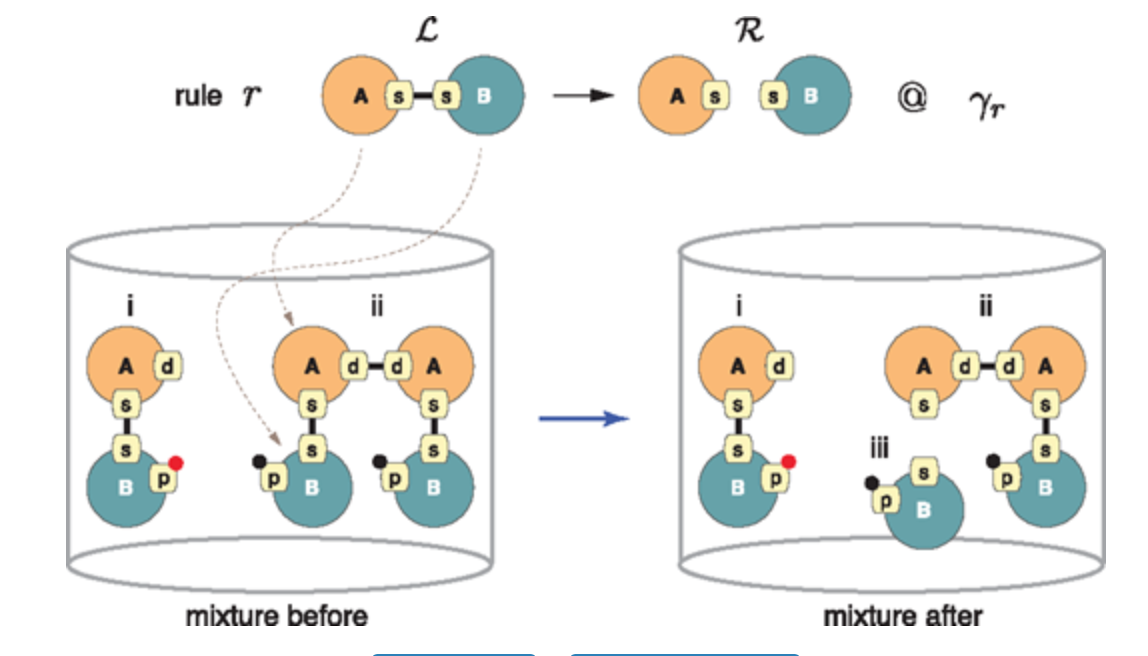
\includegraphics[width=\linewidth,height=10cm,keepaspectratio]{mixture.png}	
	\caption{Application of rule `r' to a reaction mixture \textswab{M} , comprising of two agents. $L_r$ and $R_r$ represent the state of the site graph before and after the application of rule `r'  respectively. Source: \cite{kappaPlatform}}
	\label{fig:mixture}
\end{figure}

Modeling tools built using latest technology help to visualize the protein interactions. Some examples of this include Virtual Cell \cite{vcell} and Kappa Simulator KaSim \cite{kasim}, which provide an environment for the modeling and simulation of cellular interactions. The Kappa rules can be fed into KaSim, which is a protein interaction simulator that implements continuous time Monte–Carlo algorithm (CTMC). Similarly, the rules created in BioNetGet \cite{bioNetGen} format can be simulated with NFsim \cite{nfsim}. KaSim and NFsim employ the process of stochastic modeling that can be used to describe highly complex interactions. Besides them there also exist other stochastic modeling tools like STOCHSIM \cite{stochsim}, which can be used by researchers, to compare the results.

In addition to KaSim, the Kappa simulator, there are tools like KaSA (Kappa Static Analyzer) and KaSTOR (Kappa Story Extractor). As per \cite{kappaPlatform}, KaSA helps in analyzing the static properties of the model that can help in debugging, as it can efficiently detect discrepancies between actual and expected behavior. KaSA relies on a technique called `abstract interpretation' described in \cite{kappaPlatform} to achieve this task. KaSTOR helps by providing an insight as to how an event of interest EOI was obtained in a particular event trace. EOI is obtained by the simulation of a model. KaSTOR works on the concept of mechanistic causality in molecular systems. KaSim generates an output called `trace' which is a sequence of events generated as a result of the simulation. Algorithms such as the one stated in \cite{danos2012graphs} aid this process. This is dealt in greater detail, in the Analysis of KaSim outputs, subsection.

\subsection{Syntax and semantics of Kappa rules}
Kappa rules are formally documented well. Their specification and syntax can be found in \cite{kasim} and \cite{kappaURL}. In rule based specifications graphs are formally specified as objects which have been converted to a notation of textual form, for convenience. As per these rules an agent site denoted  by `s', has a binding state `n' can be specified as s[n]. Here `n' can be any positive integer or may be replaced by a `.', which indicates the site is not bound. In case `n' is a positive integer then it implies that the site is bound to another unique site having the same binding site `n', within the same PPI expression. Hence, a sub expression like, (Agent1 [site1 [1]], Agent2 [site2 [1]] ) indicates that Agent1 is bound to Agent2 through site1 of Agent1 and site2 of Agent2. The protein sites may also have their own internal states which is specified within curly brackets `\{\}'. Hence Agent1(site1\{p\}[.]), implies that Agent1 has an unbound site name site1 that is in an internal phosphorylated state (denoted by `p'). 

Figure \ref{fig:kappa}, depicts the process of obtaining a Protein interaction rule from the textual information of research literature. These rules when passed to KaSim, the Kappa simulator help to visualize the PPI interactions. 

\begin{figure}[H]
	\centering
	\captionsetup{justification=centering}
	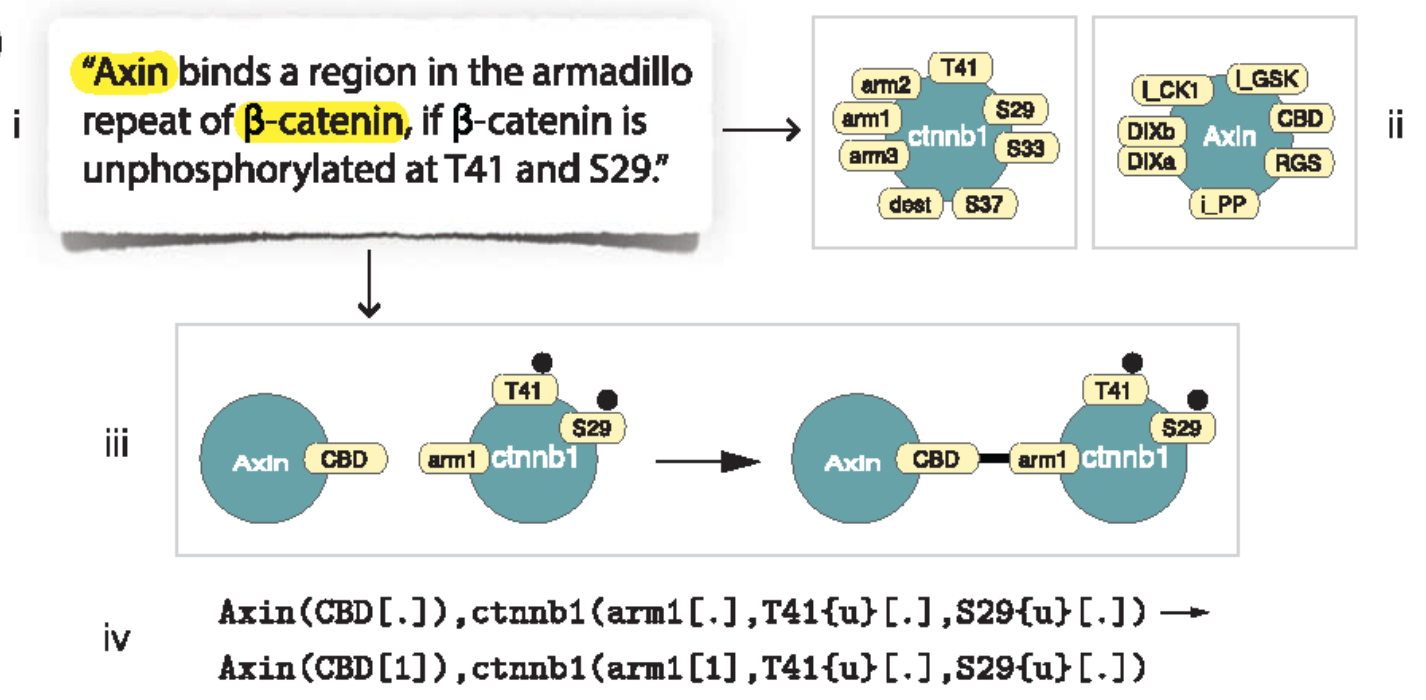
\includegraphics[width=\linewidth,height=10cm,keepaspectratio]{kappa.png}	
	\caption{Depiction of obtaining a Protein-Protein interaction (PPI) rule from research literature. Source: \cite{kappaPlatform}}
	\label{fig:kappa}
\end{figure}

\subsection{Analysis of KaSim outputs}
As per \cite{kappaPlatform}, KaSim generates as it's output the whole sequence of events called trace. The analysis of KaSim output includes discovery of the path by which a particular event of interest (EOI) has occurred. The problem can be formally stated as follows: \\
Provided a trace of events denoted by $\tau$, where $\tau$ = $e_1,e_2,..e_n$ and $e_n$ denotes an individual event. The problem is to find a suitable explanation for an EOI, where the EOI is an event, $e_n \in$ $\tau$ = $e_1,e_2,..e_n$. This process is called causal analysis and in Kappa platform KaSTOR, the software agent is utilized for this purpose. The working of this software and the process of causal analysis, is elucidated using the following figure, \ref{fig:eoi}
\begin{figure}[H]
	\centering
	\captionsetup{justification=centering}
	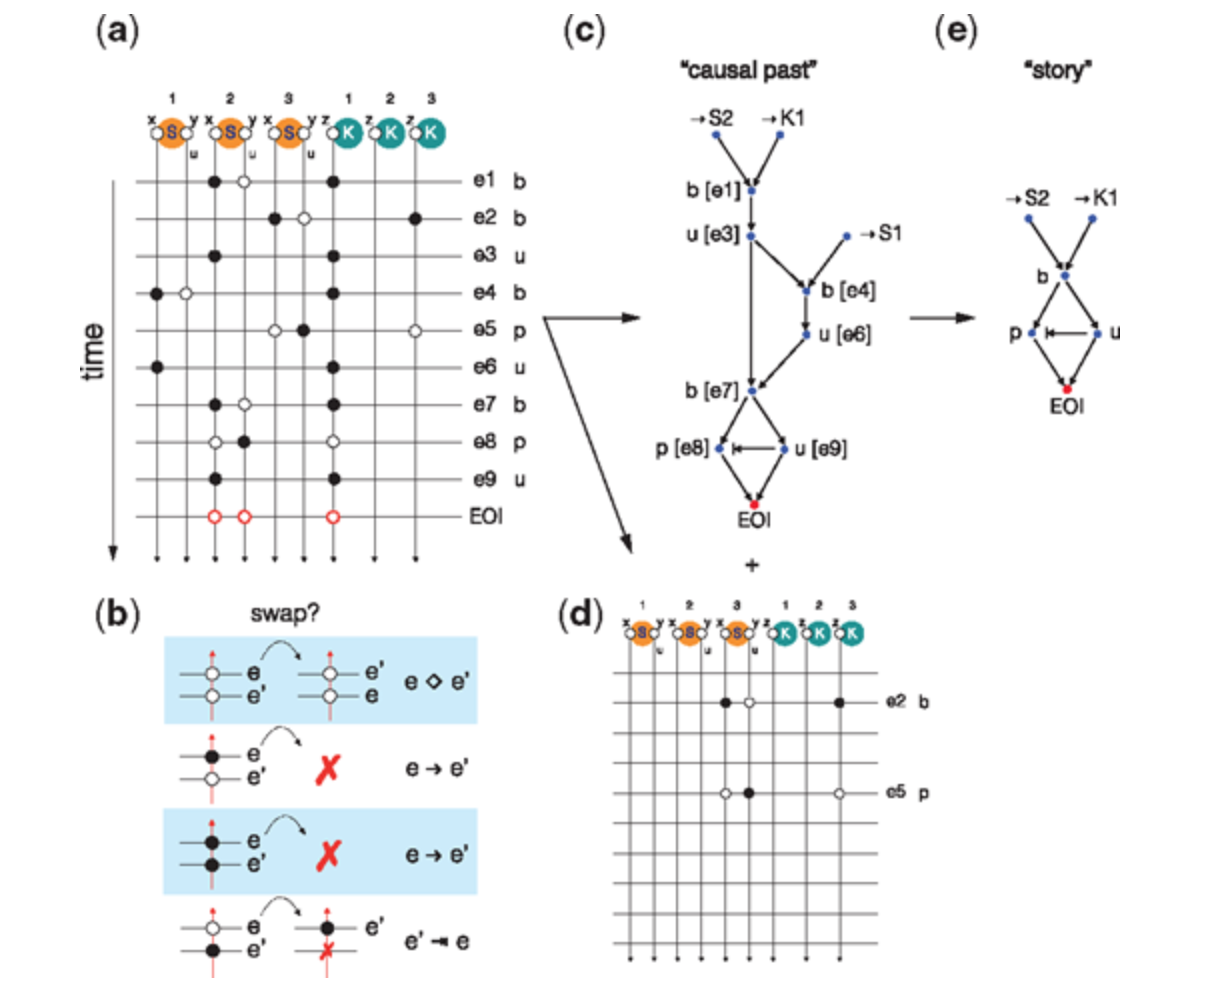
\includegraphics[width=\linewidth,height=10cm,keepaspectratio]{eoi.png}	
	\caption{Explanation of causal analysis. Source: \cite{kappaPlatform}}
	\label{fig:eoi}
\end{figure}

In figure \ref{fig:eoi} (a), the vertical lines from each site, of every agent within the mixture denotes a thread. This thread contains the record whether an event tested or modified the state of a site. It should be noted that in kappa terminology a modification of site also implies a test. The events are shown with the horizontal markings. The black discs denote that the thread was modified by its corresponding horizontal event and the white circle denotes that the thread was tested.

As per \cite{kappaPlatform}, causality comprises of a relation between events. The algorithm begins by reconstructing the causal past of `*', the identity rule. The figure \ref{fig:eoi} (b) depicts an event `e' that is followed by event ` e$'$ '. and iteratively quries if the modification or test of the site in e$'$  could have occurred before `e'. There are certain rules for the query which are detailed in \cite{kappaPlatform}, under causal linages and compression. This procedure results in a directed acyclic graph (DAG) as shown in \ref{fig:eoi} (c) which represents the precedence structure of the causal past. The procedure depicted in \ref{fig:eoi} (b) also eliminates from within the trace, any events irrelevant to the EOI. This is shown in figure \ref{fig:eoi} (d). The problem with obtaining the precedence structure is that it may violate a property called `necessity'. A method to tackle this problem involves an algorithm called minimization causal compression elaborated in \cite{danos2012graphs}. KasTOR translates the causal past into a boolean expression where each event is associated with a Boolean variable. The processing within KasTOR results to a compressed form of the causal past as shown in the figure \ref{fig:eoi} (e).

\section{Application of Protein-Protein Rule Interaction Database}
The databse for PPIs stored in a rule based format will have several applications. Some of these are covered in this section.
\begin{itemize}
	\item
	\textbf{Building the rule based model in a Kappa format:} The database will allow to build the executable rule based model based on the proteins of interest. For that, the list of proteins submitted to the database would result in a list of the relevant rule PPIs retrived as a csv file. Those rules could be built into Kappa model and simulated by KaSIM to obtain the dynamics of the molecular complex of the interest. This would allow the following more specific applications.
	\item
	\textbf{Assessment of protein druggability:} As per \cite{druggability}, ruled based PPI stored in a database are useful in the development of a rule-based model for the assessment of protein druggability. Selection of target is an important step for the discovery of drugs. The effectiveness of a drug target depends upon factors like  its chemical influence and biological importance. Druggability is defined as the ability of a target to bind a drug-like molecule with an affinity that is at a therapeutically useful level. \cite{druggability} develops a set of simple rules that govern the process of durggability which can be applied in the future to get an idea of the chemical influence of prospective targets. These rules are based on the property space of druggable pockets like volume, depth and so on.
	\item 
	\textbf{Drug effect pathway analysis:} Pathway analysis involves the study of specific molecular pathways using formalism that are qualitative and quantitative. This domain provides a tremendous computational complexity and experimental approaches that incur a high cost. Research conducted in \cite{ruleMultiscale}, included extraction of about 200 rules, related to type 2 diabetes obtained from varied sources like literature, pathway databases and conversion from different kinds of models. Using these rules \cite{ruleMultiscale} a multi-scale rule-based modeling platform was constructed. This modeling platform was then used for simulation of drug effect pathways of type 2 diabetes drugs and check for it's efficacy. The research concluded that their simulation helped in identifying effective drug combinations and provide a new way to effectively apply existing drugs for new targets.
	\item
	\textbf{Application of rule based models in biology:} Rule based models can be applied to describe the dynamics of population in a predator-prey ecosystem and simulate rhythm changes that are circadian (\cite{rule_based}).
\end{itemize}

All these research applications help in substantiating the claim that database for storing PPI in a rule format is an important tool for the study the protein complexes, drug discovery and pathway analysis aimed to improve our understanding of complex biological systems.
 

\chapter{Method}
This chapter includes the methodology adopted for the creation of rule-based Protein-Protein Interaction (PPI) database and the steps to add a new rule to it. It also contains a description of the stored procedures used to extract protein interaction rules based on either agent name or domain name pair. The source code for this project is available on an online repository (Github). This chapter contains a description of the files and folder structure within it. 

As a part of this project, a web application using Django \cite{django} was created to access the PPI rules by calling the stored procedures from within it. Chapter 3 includes the design and implementation details for the web application used to access the PPI rules. The PPI rules can be accessed from the web application, either based on the agent name or a domain name pair. 

This chapter also includes the steps for deploying the database scripts to a database server and the web application to a web server. During the process of deployment, it is often useful to have the software versions that were initially used to create the software. These are included in Appendix A, under the Software Version section. Having these details will enable developers to debug when deploying the application.

\section{Methodology for creating the database}
PPI rules were collected and provided by researchers in the form of an Excel Sheet (rule\_baseV0.2.xlsx). To extract the agent , domain names and rules from the dataset, excel sheet parser scripts were created in Python. Python scripts were also written to create and validate entity relations within the database. Description of these scripts are elucidated in Section: Description of the Project Folder and Files.

To construct the PPI database it was decided to structure the data into separate tables consisting of the agent, domain and the PPI rules. In order to connect the data in these three main tables, 2 relationship tables consisting of domain\_agent and rule\_domain\_agent were created.

 It should be noted that main tables contain certain `meta data columns'. These meta data column help in keeping track of the associated data for an entity within the table. For example, the domain table has agent\_name column, which keeps a record of all the agent\_names that it associates to. However, the correct procedure to obtain the agent\_names that associate with a particular domain is to use the domain\_agent relationship table. The Entity Relationship (ER) diagram of the database and the description of the database tables are presented in the following sections.
  \subsection{Entity Relationship Diagram:}
  \begin{figure}[H]
  	\centering
  	\captionsetup{justification=centering}
  	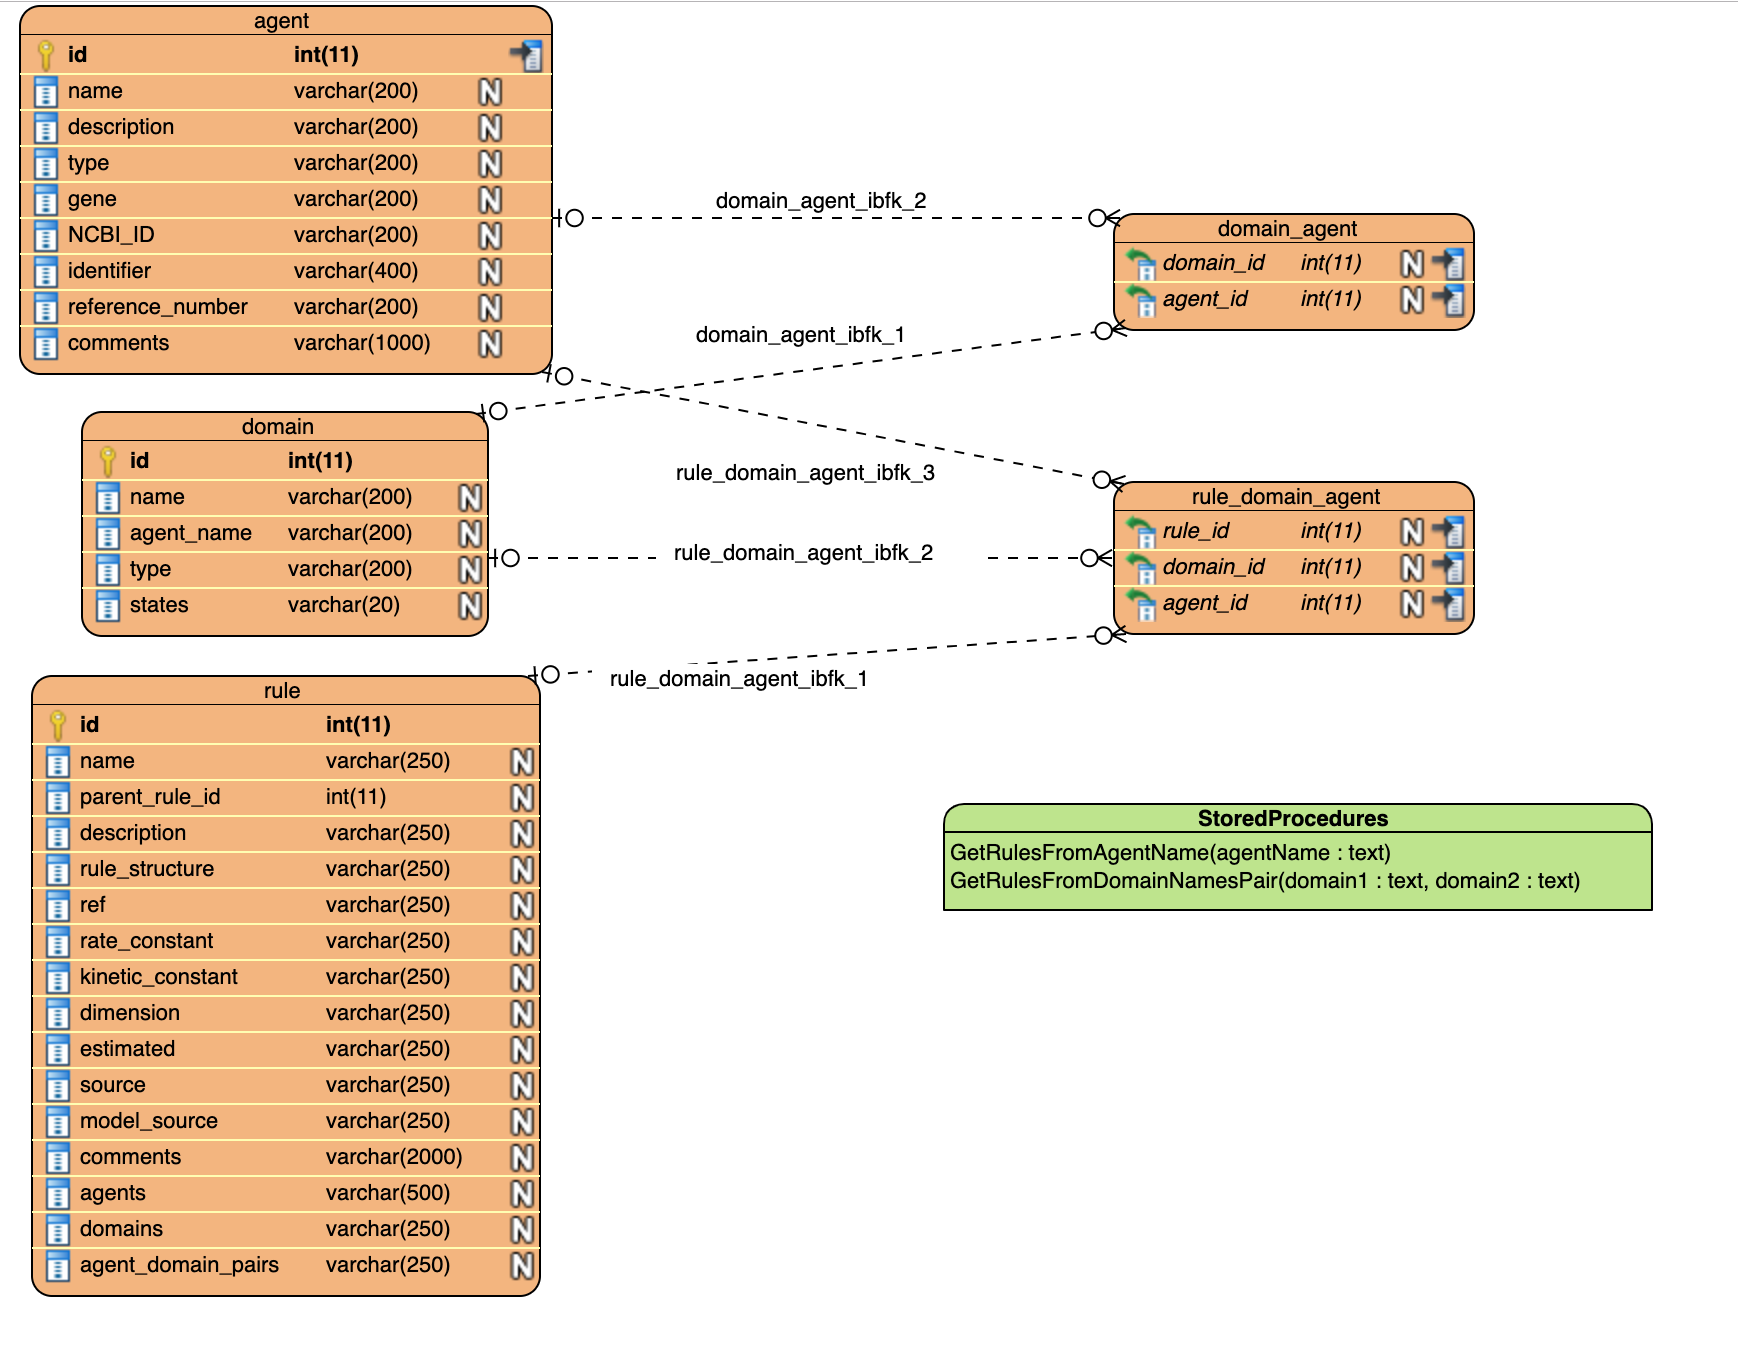
\includegraphics[width=\linewidth,height=14cm,keepaspectratio]{er.png}	
  	\caption{ER Diagram of the database}
  	\label{fig:er}		
  \end{figure}
  In Fig \ref{fig:er}, the dotted lines depict the primary-foreign key relations between the tables. The green box depicts the names of the stored procedures that are part of the database.
 \subsection{Description of  main tables}
\begin{enumerate}
	\item \textbf{agent:-} Provides a description of the protein molecule (the agent). This table contains the following fields: id, name, description, type, gene, NCBI\_ID, identifier, reference\_number and comments.
	\begin{enumerate}
		\item id: The unique identifier for the agent molecule.
		\item name: The name of the agent.
		\item description: A description of the agent.
		\item type: The type/family of the agent.
		\item gene: The particular gene
		\item NCBI\_ID, identifier, reference\_number: Provided within the dataset and contains references to the Uniprot Prosite Database \cite{Uniprot-Prosite} and literature.
		\item comments: Contains additional comments about the agent.
	\end{enumerate}
	\item \textbf{domain:-}  Provides a description of the domains that associate with the agents. This table contains the following fields: id, name, agent\_name, type, states. 	
		\begin{enumerate}
		\item id: The unique identifier for the domain name.
		\item name: The name of the domain.
		\item agent\_name: A `meta data column' that contains the names of agent molecules that associate with the particular domain.
		\item type: The type of the domain.
		\item states: Contains the possible states of the domain.
	\end{enumerate}
	\item \textbf{rule:-} Provides a description of the PPI rules within the database. 
	This table contains the following fields: id, name, parent\_rule\_id, description, rule\_structure, ref, rate\_constant, kinetic\_constant, dimension, estimated, source, model\_source, comments, agents, domains and agent\_domain\_pairs.
	\begin{enumerate}
	\item id: The Unique identifier for the rule
	\item name: The name of the rule
	\item parent\_rule\_id: In some cases the rules can be traced to a parent. This field stored the id of that parent rule. By default it is 0, which signifies no parent rule.
	\item description: A description of the rule.
	\item rule\_structure: The structure of the rule. 
	\item ref, source: A reference to the rule.
	\item rate\_constant: The rate constant for the reaction.
	\item kinetic\_constant: The kinetic constant may contain numerical value or a formula to which the rate\_constant can be plugged to obtain the result.
	\item dimension: The dimension of the reaction.
	\item estimated: The estimated value of the reaction.
	\item model\_source: A reference to the model from which the PPI is obtained.
	\item comments: Any additional comments about the rule.
	\item agents: A `meta data column' containing the names of the agent molecules that take part in the rule.
	\item domains:A `meta data column' containing the names of the domains that take part in the rule.
	\item agent\_domain\_pairs:	A `meta data column' containing the names agent and associated domains that form a part of the protein interaction.
	\end{enumerate}
\end{enumerate}

 \subsection{Description of  relationship tables}
\begin{enumerate}
	\item \textbf{domain\_agent:-} Each row contains the id of a domain and the id of an agent, obtained by referencing the domain and agent table respectively. 
	By obtaining the domain id from the domain table, the corresponding agent ids that associate with the domain can be obtained. This can then be used to obtain the agent names that associate with that particular domain.
	\begin{enumerate}
		\item domain\_id: The Id of a domain (from domain table).
		\item agent\_id: The Id of an agent (from agent table).
	\end{enumerate}

	\item \textbf{rule\_domain\_agent:-} Each row contains the id of a rule, id of a domain and the id of an agent, obtained by referencing the rule, domain and agent table respectively. Hence, this table connects the agents and domains to the PPI rules from the rule table in the database.
	\begin{enumerate}
		\item rule\_id: The Id of a rule (from rule table).
		\item domain\_id: The Id of a domain (from domain table).
		\item agent\_id: The Id of an agent (from agent table).
	\end{enumerate}
\end{enumerate}
 \subsection{Advantages and  disadvantages of the database structure}
 \subsubsection{Advantages}
The database structure is optimized for fast read operations. This is because, by using the id structure to uniquely identify entities in the database, we can leverage the power of indexing \cite{indexing}, which can be used to obtain the results faster. As per \cite{indexing}, in section 8.3.1, most MySQL indexes like primary key, unique key are stored in B Trees. Due to this, it is possible to obtain rows matching the where clause quickly and even leverage the power of Multiple-Column Indexes, as per \cite{indexing} section 8.3.6. It was also verified in MySQL workbench that the relationship tables (domain\_agent and rule\_domain\_agent) had each of the columns indexed as a B Tree. Hence MySQL would internally be able to work more efficiently with this structure than we if we employed a method that included string regex based searching.
 \subsubsection{Disadvantages}
 The disadvantage of this database design is that it makes the write operations a multi-step process. For example, if we wanted to add a new rule to the database then besides performing the regular checks, several entries may have to be made in different tables within the database. This is however not a major disadvantage as the database is expected to have many more read operations than write, also the next section states the steps to add a new PPI rule to the database. While trying to make a new entry within the database, following these rules will help in reducing the errors.
\section{Steps for adding new entries to the database}
\subsection{Agent}
	Query the agent table and check if an agent exists with the given name. It should be noted that the agent name is case sensitive. In case it exists then there is no need to add a new entry to the database. However, if it does not exist then a new entry can be made in agent table filling in the relevant fields. 
\subsection{Domain}
	Query the domain table and check if a domain exists with the given name. It should be noted that the domain name is case sensitive. In case it exists then there is no need to add a new entry to the database. However, if it does not exist then a new entry can be made in domain table filling in the relevant fields. 
\subsection{Domain-Agent Relationship}
	When the Agent/Domain is added to the database to connect them we have to make entries within the domain\_agent table. Based on the entries made in the Agent and Domain table we can obtain the corresponding ids and make entries containing the (domain id, agent id) pairs. If a new agent is added then all its corresponding domains need to be entered as separate rows where the agent id will remain the same. If a new domain is added then all its corresponding agents need to be added as separate rows where the domain id will remain the same. 	
	It should be kept in mind that if a new agent is added to the agent table and it has a new corresponding domain added to the domain table, then that pair must be entered only once within the domain\_agent table.	
\subsection{Rule}
	To add a new rule to the database, first check if the rule already exists within the database. If not, then obtain the agents and domains that take part in the rule. Verify that the necessary agents, domains and domain\_agent entries exist within the database. If not, then first make the necessary entries in these three tables as per guidelines in the previous sections. Then add the PPI rule to the rule table in the database. 
	\subsection{Rule-Domain-Agent}
	After following the steps laid out in Rule subsection, the three pair tuple/s consisting of the rule\_id, agent\_id for each of the agents in the rule and the domain\_id for each of the domains that associate with the corresponding agent within rule, need to be entered in the rule\_domain\_agent table as (rule id, domain id, agent id).
\section{Description of Stored Procedures}
\section{Description of the Project Folder and Files}
\section{Web Application for accessing the stored procedures}
\section{Deployment steps}
\subsection{Database Scripts}
\subsection{Web Application}

\chapter{Results and Discussion}

\chapter{Conclusions}

\section{Final Reminder}

The body of your dissertation, before the references and any appendices,
\emph{must} finish by page~40. The introduction, after preliminary material,
should have started on page~1.

You may not change the dissertation format (e.g., reduce the font
size, change the margins, or reduce the line spacing from the default
1.5 spacing). Over length or incorrectly-formatted dissertations will
not be accepted and you would have to modify your dissertation and
resubmit.  You cannot assume we will check your submission before the
final deadline and if it requires resubmission after the deadline to
conform to the page and style requirements you will be subject to the
usual late penalties based on your final submission time.


\bibliographystyle{plain}
\bibliography{mybibfile}

%% You can include appendices like this:
 \appendix
% 
\chapter{Software Version}
% 
This section includes software versions that were used to create and deploy the application onto a local machine. While deploying to a database/web server it may be helpful to have these details.
 \section{Operating System}
 \section{MySQL Version/ Client Version}
 \section{Python Version}
 \section{MySQL Connector Version in Python scripts}
 \section{Django Version}
 \section{Data Tables Version}
\end{document}
